\begin{frame}
\frametitle{Results from dEDM precursor experiment}
\framesubtitle{Precursor I: 3 maps with initial-slope method (IS). Precursor II: 2 maps IS + 5 maps with PB}

\vspace{-0.1cm}
\textbf{EDM resonance strength map for $\varepsilon^\text{EDM}$, includes tilts of invariant spin axis due to EDM and magnetic ring imperfections.}

\begin{columns}[T]
\column{0.45\textwidth}
\vspace{-0.2cm}
\begin{center}
	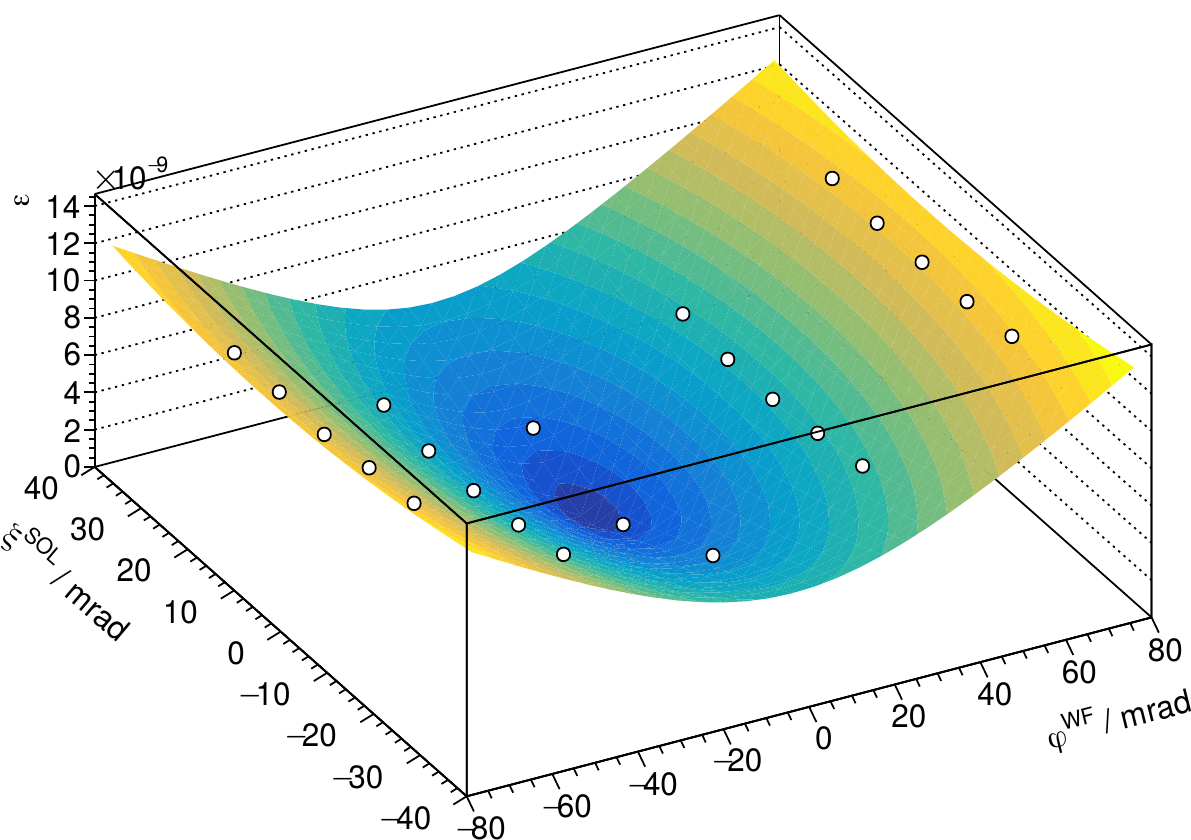
\includegraphics[width=0.7\textwidth]{map4.png}
	\vspace*{-20ex}\hspace*{-1.5cm}  % Tune this to the image height.
	\begin{center}
		\textcolor{red}{preliminary}
	\end{center}
	\vspace*{20ex}\hspace*{1.5cm}
\end{center}
\vspace{-0.2cm}
\column{0.55\textwidth}
Determination of minimum via fit with theoretical surface function yields: 
\begin{itemize}
	\item $\color{ForestGreen}{\boxed{\phi_0^\text{WF} / \text{mrad} = 2.51 \pm 0.04}}$ 
	\item  $\color{Maroon}{\boxed{\xi_0^\text{Sol} / \text{mrad} = -3.93  \pm 0.06}}$
\end{itemize}
\small Analysis by Vera Shmakova and Achim Andres
\end{columns}	

\vspace{-1.4cm}
\begin{block}{\small \textbf{Extraction of deuteron EDM:}}
\vspace{-0.1cm}	\begin{enumerate}
	\item Minimum determines spin rotation axis (3-vector) at RF WF, \textit{including EDM}.
	\item Spin tracking in COSY lattice $\rightarrow$ orientation of stable spin axis \textit{w/o} EDM.
	\item EDM is obtained from the difference of 1.\ and 2.
\end{enumerate}
\end{block}

\vspace{-0.3cm}
\begin{alertblock}{\small \textbf{EDM analysis now focuses more on systematics}}
\begin{itemize}
	\item Data analysis close to final \& EDM results in preparation.
	\item Goal: Describe observed tilts of stable spin axis by spin tracking. 
\end{itemize}
\end{alertblock}

\end{frame}
